\documentclass[tikz,border=4pt]{standalone}
% Estilo común de los diagramas de bloques (se usa con \input en cada standalone)
\usepackage[defaultsans,scale=0.92]{lato}
\usepackage{libertinust1math}
\usepackage{xcolor,amsmath}
\usepackage{tikz}
\usetikzlibrary{positioning,arrows.meta,calc,shapes.geometric}
\usepackage{../../notacion}
\definecolor{ctrlazul}{HTML}{1E5AA8}\definecolor{ctrlnoche}{HTML}{14213D}
\definecolor{ctrlcoral}{HTML}{D1495B}\definecolor{ctrlverde}{HTML}{2A9D8F}
\definecolor{ctrlambar}{HTML}{E09F3E}\definecolor{ctrlgris}{HTML}{5C677D}
\definecolor{ctrlvioleta}{HTML}{6C4AB6}\definecolor{ctrlteal}{HTML}{0F7173}
\tikzset{
  >={Stealth[length=2.4mm]}, every node/.style={font=\small},
  bloque/.style={draw=ctrlnoche,fill=ctrlazul!7,thick,rounded corners=1.5pt,minimum height=9mm,minimum width=13mm,inner sep=4pt},
  suma/.style={draw=ctrlnoche,thick,circle,inner sep=0pt,minimum size=6mm},
  senal/.style={->,thick,draw=ctrlnoche},
  rot/.style={font=\footnotesize,text=ctrlgris},
}

\begin{document}
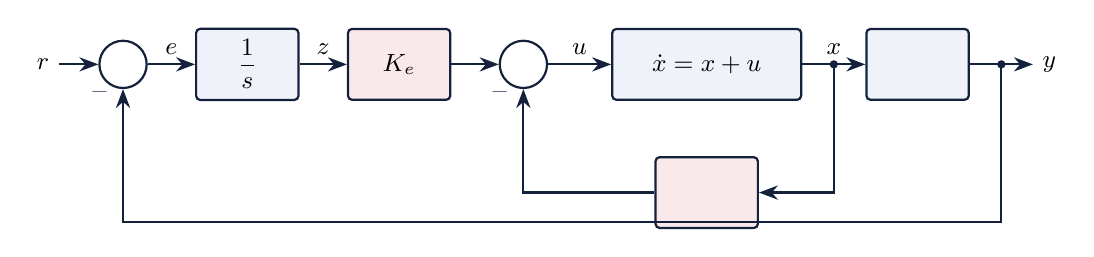
\begin{tikzpicture}[node distance=8mm]
  \node (r) {$r$}; \node[suma,right=5mm of r] (S1) {};
  \node[bloque,right=6mm of S1] (I) {$\dfrac1s$};
  \node[bloque,right=6mm of I,fill=ctrlcoral!12] (Ke) {$K_e$};
  \node[suma,right=6mm of Ke] (S2) {};
  \node[bloque,right=8mm of S2,minimum width=24mm] (P) {$\dot x=\Am x+\Bm u$};
  \node[bloque,right=8mm of P] (C) {$\Cm$};
  \node[right=8mm of C] (y) {$y$};
  \coordinate (nx) at ($(P.east)!0.5!(C.west)$); \coordinate (ny) at ($(C.east)!0.5!(y.west)$);
  \node[bloque,below=7mm of P,fill=ctrlcoral!12] (K) {$\Km$};
  \draw[senal] (r)--(S1); \draw[senal] (S1)--node[above]{$e$}(I); \draw[senal] (I)--node[above]{$z$}(Ke); \draw[senal] (Ke)--(S2);
  \draw[senal] (S2)--node[above]{$u$}(P); \draw[senal] (P)--(C); \draw[senal] (C)--(y);
  \fill[ctrlnoche] (nx) circle (1.5pt) (ny) circle (1.5pt); \node[above] at (nx) {$x$};
  \draw[senal] (nx)|-(K); \draw[senal] (K)-|(S2);
  \draw[senal] (ny)--++(0,-20mm)-|(S1);
  \node[rot] at ($(S1)+(-3mm,-3.5mm)$) {$-$}; \node[rot] at ($(S2)+(-3mm,-3.5mm)$) {$-$};
\end{tikzpicture}
\end{document}
